\cleardoublepage
\chapter{绪论}

\section{研究背景及意义}
近年来,物联网(Internet of Things,IoT)技术的快速发展正在逐渐改变人们的生活和工作方式,其应用范围覆盖了农业、制造业、医疗保健、零售业和公用事业等多个领域。
随着物联网技术的不断进步和应用领域的拓展,可以预见,未来将有越来越多的设备加入互联网。
如\autoref{fig:iot}所示,根据Gartner的分析~\cite{hung2017leading},2027年将有三千亿物联网设备接入网络。
这些设备产生的离散数据将达到泽字节(ZettaBytes, ZB)~\cite{al2020internet},这一数字预示着未来数据的爆炸式增长,形成庞大的数据海洋。

\begin{figure}[t]
    \centering
    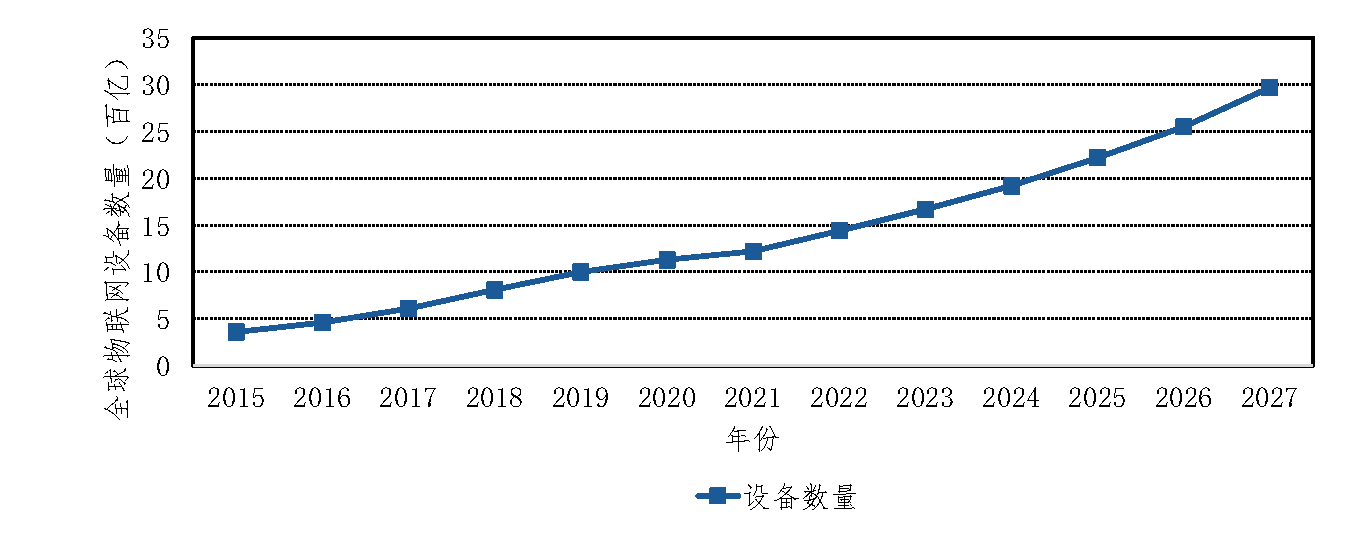
\includegraphics[width=1\linewidth]{figures/timechain/iot.pdf}
    \caption{2015-2027年全球物联网设备预测数量}
    \label{fig:iot}
\end{figure}

面对如此大规模的数据增长,如果使用传统的集中式服务器管理方式,如AWS IoT~\cite{aws}、阿里云~\cite{aliyun}等,可能会带来诸多挑战。
这些挑战中最为突出的是单点故障问题~\cite{gill2011understanding},即所有数据都集中在一个或几个服务器上,一旦这些中心节点发生故障,整个系统的稳定性和可用性将受到严重影响,甚至可能导致数据的不可用或丢失。
此外,集中式存储方案在数据传输效率、扩展性和维护成本方面也存在一定的局限性。
这些问题限制了集中式存储系统在处理大规模、高动态物联网数据时的灵活性和效率。

分布式数据库如Apache Cassandra~\cite{lakshman2010cassandra}、Spanner~\cite{corbett2013spanner}、Ceph~\cite{weil2006ceph}等,可以解决单点故障问题。
但是它们在需要高度透明的多方共享数据场景中,如金融交易和医疗记录,这些分布式数据库容易受到恶意合作者的数据篡改攻击,从而直接威胁到数据的完整性和安全性。
例如,在2024年,十堰市某重点排污单位篡改在线监测数据以逃避监管~\cite{example},产生了严重的环境影响和经济损失。
因此,开发一种既能够提供高可靠性、又能够确保数据安全性的存储解决方案,对于物联网数据的管理和保护至关重要。

区块链技术~\cite{houy2014bitcoin}以其可追溯性和不变性为特征,为解决集中式存储的单点故障问题和分布式数据库的恶意篡改问题提供了新的途径。
区块链通过将数据存储在去中心化的账本中,并利用共识协议来解决各个节点之间可能发生的冲突,从而增强了数据的安全性和透明度,降低了成本,并支持节点间的平等协作。
这种去中心化的数据存储方式,使得任何一个节点的故障都不会影响整个系统的运行,从而有效避免了单点故障的风险。
同时,区块链的不可篡改性确保了数据一旦被记录,就无法被更改或删除,这对于需要高度数据完整性的应用场景尤为重要。

然而,基于区块链的存储系统也面临着挑战。
由于其较低的交易处理速度和较高的计算要求~\cite{dorri2017towards},区块链技术目前主要应用于价值巨大但数据密度较低的领域,如金融服务、供应链管理等。
但是,对于面向生成频率快、数据体量大的物联网时序数据的应用,如智能城市、工业自动化等,区块链技术的性能瓶颈限制了其广泛应用。
因此,如何优化区块链技术,提高其处理速度和效率,使其能够更好地服务于物联网数据的存储和管理,是当前研究和开发的重要方向。

目前,有许多研究人员致力于提高基于区块链的存储系统的性能。
根据数据的存储位置,这些工作可以分为两类,即链上存储和链下存储。

对于链上存储,数据作为存储在区块链上的交易记录的一部分。
用户通过区块链中的索引,即默克尔树来获取这些数据。
现有工作通过提供用户友好的查询语言~\cite{zhu2019sebdb,xu2019vchain,wang2022vchain+}提高了系统可用性,并通过改进索引方案~\cite{li2023lvmt,zhang2024cole}、区块链存储分片~\cite{zamani2018rapidchain,hong2023gridb,el2019blockchaindb}等方式提高系统吞吐量。
然而,在链上存储物联网时序数据的开销非常高。
对于大量且快速生成的物联网时序数据,将其连续存储在区块链上需要实现共识和账本复制的过程,这可能会导致巨大的存储压力和通信开销。
因此,物联网数据存储的一种更实用的方法是使用链下存储方案。

对于链下存储,数据存储在区块链之外的存储节点,区块链只存储必要的元数据或对数据的引用,如哈希或加密指针。
链下存储提供了比链上解决方案更大的可扩展性和更低的成本,因此业界和学术界对链下存储方案非常感兴趣,产生了例如Storj~\cite{storj2018storj}、BigchainDB~\cite{mcconaghy2016bigchaindb}、Sia~\cite{sia}等项目。
然而,现有的工作大多是为存储大文件而设计的。
相比于较大的物联网视频流数据,物联网时序数据的产生频率快、数据体量大,在区块链中存储每个离散数据项的哈希值将产生难以接受的开销。
此外,物联网应用场景通常需要存储系统支持高效查询(例如聚合查询),而现有的基于文件的存储系统不支持这一点。

本文基于链下存储的方案,提出了一种面向物联网的区块链存储系统,并基于该系统进行了一系列广泛的测量。
针对测量中发现的低效查询性能问题,本文提出了TimeChain,一个基于区块链的物联网时序数据高效可信存储系统。
TimeChain分别针对测量中发现的三个性能根因提出了自适应聚合机制、基于共识的存储节点选择机制和基于局部敏感哈希树的数据完整性验证机制。
实验结果表明,TimeChain相比现有的基于区块链的存储系统有显著的性能提升,对于实现物联网数据的可信高效存储具有一定的理论和实践价值。

\section{论文主要工作}
为了对海量物联网数据进行可信、高效的存储,受链下存储方案的启发,本文提出了一种基于区块链的物联网时序数据基本存储方案。
该方案将数据聚合成多个批处理单元,仅将每批数据的哈希值存储在链上,并将完整的原始数据保存在链外。
这种批处理存储方法大大减少了数据开销。

本文基于Hyperledger Fabric~\cite{hyperledger}和星际文件系统(InterPlanetary File System,IPFS)~\cite{benet2014ipfs}等开源组件实现了该系统,并基于YCSB数据集对该方案的性能进行了测量。
结果表明,与每个数据单独存储相比,将数据批量存储的存储延迟平均减少了37.4倍。
这种存储性能的显著提升使得区块链支持物联网数据存储成为可能。

然而,不可否认的是,这样的批处理方案会影响查询性能。
具体来说,批处理存储的平均延迟达到了165.4ms,这一延迟水平对于许多对实时性要求高的物联网应用来说是不可接受的。
以地震监测为例,其对延迟的要求是低于100ms,而在自动驾驶领域,理想的延迟更是要低于50ms。
为了深入理解这一性能瓶颈,本研究详细分析了影响查询性能的三个关键原因:

\begin{itemize}
    \item \textbf{范围查询跨越多个批处理单元。}
    在处理时间序列数据时,查询操作如范围查询、聚合查询和过滤查询等,通常涉及多个数据点。
    如果数据的批处理方式不够合理,单个查询可能需要访问多个批处理单元。
    实验结果显示,超过84.25\%的查询需要跨越至少10个批处理单元。
    当这些单元分散在不同的存储节点上时,就会增加额外的查询和传输延迟,影响整体的查询响应速度。
    
    \item \textbf{存储节点选择不当。}
    在本研究的测量中,传输延迟在总查询延迟中占据了显著的比例。
    不同地理位置的存储节点之间存在传输距离的差异,这直接影响了数据传输的延迟,选择地理位置较远的存储节点会导致传输延迟显著增加。
    此外,如果存储网络中存在恶意节点,即使所选节点的传输延迟较小,数据的完整性也可能受到威胁,从而影响数据存储服务的完整性和可靠性。

    \item \textbf{完整性证明数据量大。}
    为了使存储提供商能够快速响应数据拥有者的数据查询请求,并提供数据完整性的证明,这些证明需要与存储提供商一同存储。
    实验表明,由于原始数据本身较小,对小粒度数据哈希产生的完整性证明相对较大,在总传输数据量中占据了相当大的比例,达到了接收数据的48.8\%。
    在网络繁忙时段,大量的完整性证明数据传输会加剧网络拥塞,增加传输延迟,从而影响查询性能。
\end{itemize}

针对测量中发现性能瓶颈的三个根本原因,本文提出了TimeChain,一种高效的物联网时序数据区块链存储技术,以解决这些问题。
本文的贡献主要如下:

\begin{itemize}
    \item \textbf{在数据聚合阶段,本文提出了一种面向链下存储的自适应聚合机制。}
    为了减少范围查询过程中跨越的存储节点数量,本文通过构建自适应无向加权图,将批处理问题转化为图划分问题。
    对于该图划分问题,由于物联网数据的查询通常不遵循特定的规律,数据分布可能不会形成传统的圆形。
    因此传统方法如K-means~\cite{kanungo2002efficient}需要固定图的形状和数量,GMM~\cite{he2010laplacian}则计算复杂度较高,因此不适合物联网数据的聚合。
    由于谱聚类算法适合用于不规则形状的图划分问题,因此本文使用谱聚类算法进行子图划分,以减少聚合查询期间的节点访问次数。

    \item \textbf{在存储节点选择阶段,本文提出了一种基于共识的存储节点选择机制。}
    对于节点选择过程,本文主要考虑选择过程的正确性和安全性。
    选择过程的正确性指的是选择的节点传输时延较短、提供存储服务质量较高,选择过程的安全性则指的是决策过程本身不会受到单点故障或恶意节点的影响。
    对于选择过程的正确性,受已有方案的启发,TimeChain同时考虑存储节点信誉、剩余存储空间和传输距离。
    对于选择过程的安全性,目前已有的节点选择机制都是中心化地进行节点选择,这可能会产生单点故障和数据篡改的风险。
    考虑到共识过程中的两次信息广播过程,为了在去中心化的环境中高效地选择存储节点,本文将共识过程与节点选择相结合,借助共识的两次广播过程完成节点选择所需的信息交换,以此减少数据传输和一致性开销。

    \item \textbf{在数据验证阶段,本文提出了一种基于局部敏感哈希树的数据完整性验证机制。}
    目前区块链存储系统中常用的验证数据结构,如默克尔树,其构建过程中会产生与原始数据规模相同的哈希值,这会导致传输开销过大。
    针对该问题,本文提出了一种基于局部敏感哈希(Locality Sensitive Hashing,LSH)树的数据完整性验证机制。
    该机制利用物联网场景下相邻时间序列数据点之间的相似性,通过仅传输LSH证明的非冗余部分显著减少了完整性验证所需的数据。
\end{itemize}

本文基于开源组件实现了TimeChain,并基于此评估TimeChain的性能。
结果表明,相比于现有的基于区块链的存储系统,它平均减少了64.6\%的查询延迟和35.3\%的存储延迟。
这一显著的性能提升证明了TimeChain在提高物联网时序数据处理效率方面的优势。
此外,TimeChain在支持最大存储设备数量方面展现了良好的可扩展性。
与SEBDB和FileDES相比,TimeChain分别增加了1.63倍和3.55倍的设备支持能力。
这一结果表明,TimeChain能够适应不断增长的物联网设备数量,满足未来物联网应用的发展需求。
通过消融实验,本文进一步验证了TimeChain中自适应聚合机制、基于共识的节点选择机制和基于LSH树的验证机制对于提升系统性能的重要性。

本文的相关研究工作已被以第一作者身份被CCF A类国际会议The ACM Web Conference 2025(ACM WWW 2025)接收。
此外,本文的相关研究工作也以第二发明人(学生第一发明人)身份申请发明专利一项,目前处于实质审查阶段。

\section{全文结构}

\begin{figure}[t]
    \centering
    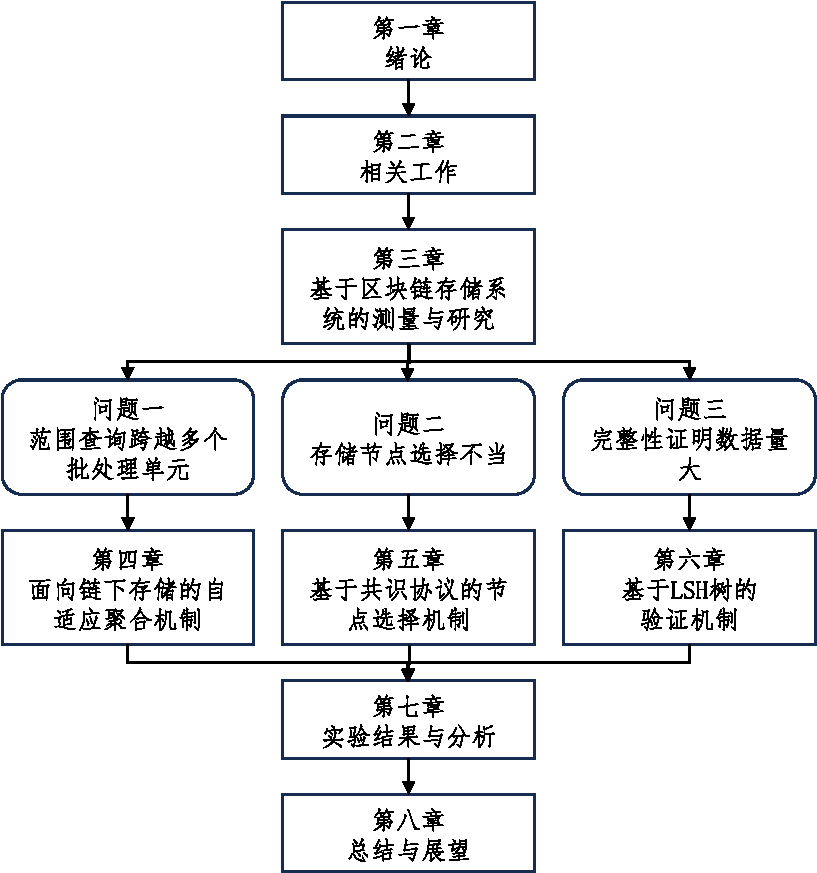
\includegraphics[width=0.8\linewidth]{figures/timechain/roadmap.pdf}
    \caption{基于区块链的物联网时序数据高效可信存储技术研究内容}
    \label{fig:roadmap}
\end{figure}

围绕上述研究内容和贡献,本文将内容分为如\autoref{fig:roadmap}所示的八个章节展开,各章节组织如下:

第一章介绍了本文的研究背景和意义,概述了本文的主要工作和贡献,以及全文的结构安排。

第二章详细回顾了中心化存储系统、分布式存储系统、区块链存储系统等相关技术领域,分析了区块链现有存储技术在本场景下的的局限性。
本文探讨了区块链链上存储机制和链下存储机制的研究进展,为本文提出的TimeChain系统提供了改进的方向和理论支持。

第三章提出了基于区块链的物联网时序数据存储系统的基础架构,并通过对系统性能的实验测量评估,揭示了现有系统的性能瓶颈。
本文进一步分析了这些瓶颈的根本原因,并提出了针对性的优化策略,提出了高效的存储技术TimeChain。
本文介绍了TimeChain的核心模块和各模块的功能,为后续章节的详细设计提供了基础。

第四章针对测量展现的跨越多个聚合单元问题,提出了一种自适应聚合机制。
本文通过构建无向加权图和采用谱聚类算法减少查询延迟,提高了数据存储的效率。
本文也进一步讨论了该机制如何根据历史查询模式动态调整数据聚合策略,以适应不断变化的查询需求。

第五章针对测量表现的存储节点选择错误问题,提出了一种基于共识协议的节点选择机制。
该机制综合考虑了节点信誉和传输距离,提高了节点选择的安全性和准确性,降低了数据传输延迟。
为了确保去中心化节点选择的效率,该机制将节点选择过程与共识过程相结合,以提高整个系统的抗攻击能力和可靠性。

第六章针对测量揭示的完整性验证数据较大问题,设计了一种基于LSH树的数据完整性验证机制。
本文利用物联网数据的局部相似性,使用LSH算法减少了验证过程中的数据传输量,提高了验证效率。
本文也进一步分析了LSH树在提高数据验证速度和减少网络负载方面的潜力,为物联网数据的高效验证提供了新的解决方案。

第七章基于开源组件实现了TimeChain,并基于公开数据集评估其性能。
本文将TimeChain与现有较为先进的解决方案进行性能对比,也通过消融实验进一步证明了TimeChain各技术点的有效性。

第八章总结了TimeChain系统的主要研究成果,并对未来的研究方向和TimeChain系统的改进进行了展望。
本文也进一步讨论了如何将TimeChain系统拓展到更广泛的应用场景,以及如何进一步提升系统性能和安全性,为后续研究提供了方向。
